\section{Métodos de muestreo de la abundancia poblacional}
\label{sec:densidad-vectorial-introduccion}

Está ampliamente aceptado que la vigilancia de Aedes aegypti es un aspecto muy importante en la
lucha contra el dengue, esta afirmación se basa en la asunción de que existe una correlación
positiva entre la densidad del vector y la enfermedad humana\cite{world2009dengue, dengueUruguayCap2}.

Muchos programas de control del dengue se basan el la utilización de índices larvarios o índices
de Stegomia, como indicadores de las densidades poblaciones de Aedes aegypti, para dirigir y
focalizar espacial y temporalmente las acciones de control del vector.

%~ * Índices de Stegomia

\subsection{Índices de Stegomia}
\label{sec:densidad-vectorial-indices-stegomia}
La Organización mundial de la salud (OMS) recomienda la utlización de tres indicadores
entomológicos, generalmente conocidos como índices de Stegomia, para estimar la densidad del
vector, Índice de casas (I.C.), Índice de Recipientes (I.R.) e Índice de Breteau (I.B.).Estos
indices son calculados a partir de muestreos de larvas y recipientes.

\subsubsection{Índice de Casas}
El índice de Casas (I.C.) es el valor numérico que especifíca el porcentaje de viviendas
infestadas con larvas, pupas o ambos estados de desarrollo del Aedes aegypti o Aedes albopictus
\cite{ibanez1995vectores, world2009dengue}, y se encuentra expresado como :

\begin{equation}
I.C. = \frac{\textit{número de casas infestadas} * 100}{\textit{número de casas inspeccionadas}}
\end{equation}

Donde :
\begin{itemize}
\item \textit{número de casas infestadas} : cantidad de casas que cuentan con al menos un contenedor que alberga a larvas o pupas de Aedes aegypti.
\item \textit{número de casas inspeccionadas} : El total de casas analizadas para el estudio.
\end{itemize}

Para este indice, se analizan los contenedores de las viviendas y alrededores, donde, se registra
como positiva cuando al menos un contenedor presenta larvas o pupas \cite{ibanez1995vectores}. Es
el de uso más generalizado para la distribución de medición de la población, pero no tiene en
cuenta el número de recipientes positivos ni la productividad de esos recipientes
\cite{world2009dengue}. Puede ser utilizado para proporcionar una indicación rápida de la
distribución del mosquito en una área determinada.

\subsubsection{Índice de Recipientes}
El índice de Recipientes es un valor numérico que consiste en el porcentaje de recipientes que
contienen agua y están infestados con las larvas o pupas del Aedes aegypti o Aedes albopictus
\cite{ibanez1995vectores, world2009dengue}, y se encuentra expresado como :

\begin{equation}
I.R. = \frac{\textit{número de contenedores positivos} * 100}{\textit{número de contenedores inspeccionadas}}
\end{equation}

Donde :
\begin{itemize}
\item \textit{número de contenedores positivos}: La cantidad de contenedores en los cuales se observan larvas o pupas de Aedes aegypti.
\item \textit{número de contenedores inspeccionadas} : El total de contenedores analizadas para el estudio.
\end{itemize}

Este índice sólo ofrece información sobre la proporción de recipientes que mantienen agua y que
son positivos \cite{world2009dengue}. Las encuestas que utilizan el índice del envase son mucho
más lentas a realizar que las encuestas sobre el índice de la casa, porque requieren que se
examinen todos los recipientes para detectar la presencia de etapas no maduras y registrar los
detalles en envases positivos y negativos para determinar su especie mediante análisis
laboratoriales.

\subsubsection{Índice de Breteau}
El índice de Breteau (I.B.) es un valor numérico que define el número recipientes con larvas,
pupas o ambos estados de desarrollo del Aedes aegypti o Aedes albopictus, que se encuentran número
de recipientes positivos por cada 100 casas inspeccionadas
\cite{ibanez1995vectores, MARQUES1993,world2009dengue}, expresada como :

\begin{equation}
I.B. = \frac{\textit{número de contenedores positivos} * 100}{\textit{número de casas inspeccionadas}}
\end{equation}

Donde :
\begin{itemize}
\item \textit{número de contenedores positivos} : La cantidad de contenedores en los cuales se observan larvas o pupas de Aedes aegypti.
\item \textit{número de casas inspeccionadas} : El total de casas analizadas para el estudio.
\end{itemize}

El índice de Breteau establece una relación entre recipientes positivos y casas, y se considera el
índice más informativo \cite{world2009dengue}.

\subsubsection{Problemática de las técnicas tradicionales}
Las técnicas tradicionales de vigilancia de Aedes aegypti utilizan índices stegomia para
determinar el grado de infestación, dispersión y densidad del mosquito en una zona y tiempo
determinados \cite{NINO2011}. La Organización Mundial de la Salud (OMS), para estimar la densidad
del vector, ha recomendado los siguientes indicadores entomológicos : Índice de Casa, Índice de
Recipiente e Índice de Breteau \cite{cenaprece2013}.

Estos índices se fundamentan en la detección de la presencia de formas inmaduras (larvas de
mosquito, pupas y restos de larvas y pupas) del vector dentro de recipientes domésticos. Un
problema es que es que los recipientes más comunes con frecuencia, no resultan ser los más
productivos \cite{world2009dengue}. Hay que tener en cuenta que la tasa de aparición de mosquitos
adultos en recipientes de gran acumulación de agua (tanques, baldes, piletas, etc), puede diferir
considerablemente de la tasa en recipientes pequeños (latas, botellas, plantas, etc), pero como
la inspección solo las registra como positivas o negativas. En consecuencia, pueden ser
clasificados como iguales, sitios con índices larvarios iguales, pero con diferentes perfiles de
recipientes, por lo tanto, las capacidades de transmisión, pueden ser bastante diferentes
\cite{world2009dengue}.

Son considerados una pobre indicación de la producción de mosquitos adultos
\cite{world2009dengue, cenaprece2013}, debido a que no reflejan la asociación que existe entre las
densidades de mosquitos y tipo de recipientes presentes, con los riesgos de transmisión de dengue
\cite{cenaprece2013}, además no se puede medir la productividad del recipiente
\cite{world2009dengue} y en consecuencia se proporciona poca o nula información de aquellas
viviendas en las que existe un mayor riesgo de presencia de mosquitos \cite{cenaprece2013}.

Actualmente, sólo son recomendados para detectar la calidad de las acciones (control de calidad)
realizadas por el personal de control larvario \cite{cenaprece2013}. Existen numerosos métodos e
indicadores más prácticos, eficientes y económicos para determinar las poblaciones de Aedes
aegypti \cite{cenaprece2013}, como larvitrampas, ovitrampas y mosquitericas.

\subsection{Larvitrampas}
\label{sec:densidad-vectorial-larvitrampas}
Las larvitrampas son, dispositivos artificiales creados con el fin de simular el habitad del
vector de forma controlada. El diseño más simple (\figref{fig:cap3-larvitrampas}) es una sección
radial de una llanta llena de agua \cite{world2009dengue}.

\begin{figure}[H]
\centering
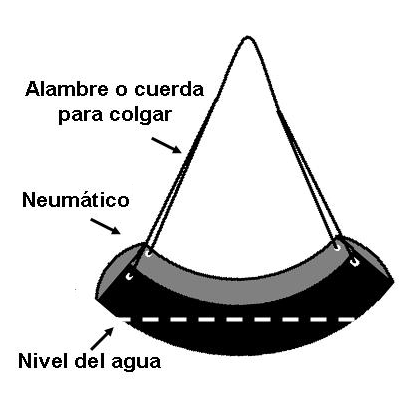
\includegraphics[width=0.4\textwidth]{capitulo-3/graphics/larvitrampa.png}
\caption{\label{fig:cap3-larvitrampas} Diseño de una larvitrampa(Tomado de
\cite{manualControlArg2009}).}
\end{figure}

Se basan en la detección del vector en su etapa, inmadura, larval
\cite{manualControlArg2009, MARQUES1993}, que brinda información sobre los patrones de actividad
espacial y estacional de ovipostura, y además, permiten reconocer las condiciones climáticas
favorables para la eclosión y desarrollo larvario \cite{manualControlArg2009}.

En las áreas infestadas, o con alto riesgo de infección con Aedes aegypti, la inspección debe
realizarse de forma periódica, según \cite{manualControlArg2009}, con el fin de :

\begin{itemize}
    \item Conocer la distribución del vector y el grado de infestación para establecer el nivel de riesgo de transmisión de dengue en las áreas geográficas infestadas.
    \item Detectar oportunamente la infestación en las áreas no infestadas.
    \item Detectar la introducción de Aedes albopictus en áreas no infestadas.
    \item Evaluación de acciones realizadas.
\end{itemize}

Las llantas o neumáticos son considerados como criaderos de alto riesgo
\cite{bisset2008distribucion, manrique1998desarrollo, ulloa1996abundancia}, donde, la
supervivencia y la duración del ciclo de vida en neumáticos son menores a los reportados para
otros tipos de contenedores \cite{manrique1998desarrollo}. Esto resalta la importancia de los
neumáticos como criaderos y blanco para el control del vector del dengue \cite{manrique1998desarrollo, ulloa1996abundancia}.

Las larvitrmpas, construidas de neumáticos, permiten transformar estos criaderos de alto
riesgo en una herramienta para el control del vector del dengue mediante el reciclaje.

\subsection{Ovitrampa}
\label{sec:densidad-vectorial-ovitrampa}
Las ovitrampas constituyen un método sensible y económico para el monitoreo del Aedes y útiles
para determinar el comportamiento poblacional del vector y conocer las áreas de riesgo
entomológico \cite{cenaprece2013}. Su diseño estándar se encuentra compuesto por una jarra de
vidrio pintada de negro \cite{dengueUruguayCap1, world2009dengue}, equipada con una chapa de
madera o paleta de madera \cite{dengueUruguayCap1, world2009dengue, website:TimothyOvitrap2014,
manualControlArg2009}. Así mismo pueden utilizarse recipientes de plástico
\cite{website:TimothyOvitrap2014, cenaprece2013, manualControlArg2009, MARQUES1993} en reemplazo
de las jarras de vidrio por su bajo costo.


\begin{figure}[H]
\centering
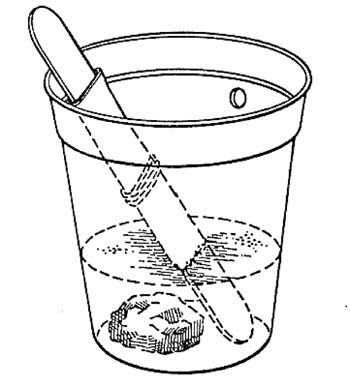
\includegraphics[width=0.3\textwidth]{capitulo-3/graphics/ovitrampa.jpg}
\caption{\label{fig:cap3-larvitrampas} Diseño de una ovitrampa (Tomado de
\cite{website:TimothyOvitrap2014}).}
\end{figure}

Las ovitrampas constituyen un método sensible y económico para el monitoreo del Aedes aegypti
\cite{cenaprece2013, world2009dengue}, y son útiles para determinar el comportamiento poblacional
del vector y conocer las áreas de riesgo entomológico \cite{cenaprece2013}. La información
proporcionada permite para determinar la distribución espacial y temporal de Aedes aegypti y otros
mosquitos \cite{dengueUruguayCap1, NINO2011}. Se pueden instalar y preparar en forma relativamente
rápida en grandes áreas \cite{world2009dengue}.



%~ * Distribución de dispositivos de ovipostura
%\section{Larvitrampas}
\label{sec:densidad-vectorial-larvitrampas}
Antes de la utilización de la larvitrampa, ésta debe cepillarse y flamearse,
luego mantenerla sumergida en agua durante no menos de tres días, para
asegurarse que el agua no contenga residuos de sustancias que puedan actuar
como larvicida. De esta manera, además, se garantiza la destrucción de
algún huevo del mosquito que estuviese previamente en el neumático o en
larvitrampas ya utilizadas.

\subsection{Especificaciones para la colocación e inspección}
Instalarla a una altura de 50 cm (del suelo a la base de la larvitrampa).
Protegerla de la luz directa del sol, el aire, la lluvia, en lugares a
media luz o completamente a la sombra. No deben ubicarse cercanas a depósitos
de agua. Debe evitarse su colocación en lugares completamente pavimentados,
u otros que tengan mucha refracción de la luz. Debe estar visible para la
hembra del mosquito. Protegerla de niños y animales domésticos (perros,
gatos, roedores, etc.)

\subsection{Forma de revisión}
Se establece una rutina semanal para revisar las larvitrampas, para lo
cual, una vez por semana debe vaciarse todo su contenido cuidadosamente
(para que no quede ninguna larva en sus paredes) en un recipiente adecuado
para realizar la inspección. En caso de ser positivas, se registra como
tal y las larvas serán colectadas en tubos para ser enviadas al laboratorio
para su determinación taxonómica. Luego, el dispositivo se lava y se acondiciona
para ser colocadas nuevamente siguiendo las especificaciones ya descritas.

\subsection{Consideración final}
Tener en cuenta que en verano, con condiciones más favorables para el
desarrollo de esta especie, las larvas pueden alcanzar el estadio de
adulto entre 6 y 7 días desde la ovipostura, por lo que es necesaria la
inspección de todas las larvitrampas en los tiempos indicados a fin de
evitar que alguna de ellas se transformen en criaderos de adultos.

%~ * Seguimiento y control de dispositivos de ovipostura
%\subsection{Ovitrampa}
\label{sec:densidad-vectorial-ovitrampa}
Son recipientes que ofrecen a las hembras de Aedes aegypti un lugar colocar
los huevos. Detecta la presencia de huevos y por lo tanto actividad de
ovipostura. Las ovitrampas consisten en frascos de plástico o pequeñas
macetas plásticas de unos 500 ml de color oscuro preferentemente, en cuyo
interior, se coloca una pieza plana de madera (baja-lengua o similar).
Asimismo, también pueden construirse con un pote de vidrio de boca ancha,
de aprox. medio litro, pintado de negro por fuera y equipado con una paleta
de cartón o madera (baja-lengua) sujeta verticalmente al interior, con su
lado áspero mirando hacia adentro. Las dimensiones del recipiente no son
críticas pero todos los frascos a usar en un estudio particular deben ser
idénticos. Al frasco se le deberá agregar 250 ml de agua limpia.

%~ * Recolección de resultados
%\section{Mosquitérica genérica}
Es un dispositivos de oviposturas más recientes, cuenta con un sencillo
diseño y de fácil fabricación debido a que los materiales necesarios para
su construcción son fácilmente accesibles.

